% This is samplepaper.tex, a sample chapter demonstrating the
% LLNCS macro package for Springer Computer Science proceedings;
% Version 2.21 of 2022/01/12
%
\documentclass[runningheads]{llncs}
%
\usepackage[T1]{fontenc}
% T1 fonts will be used to generate the final print and online PDFs,
% so please use T1 fonts in your manuscript whenever possible.
% Other font encondings may result in incorrect characters.
%
\usepackage{graphicx}
% Used for displaying a sample figure. If possible, figure files should
% be included in EPS format.
%
% If you use the hyperref package, please uncomment the following two lines
% to display URLs in blue roman font according to Springer's eBook style:
%\usepackage{color}
%\renewcommand\UrlFont{\color{blue}\rmfamily}
%\urlstyle{rm}
%

% Olivier
\usepackage{changepage}
\usepackage{amssymb}
% \newcommand{\doublecheck}{\stackon{\checkmark\hspace{-0.3em}}{\checkmark}}
\newcommand{\doublecheck}{\checkmark\hspace{-0.5em}\checkmark}


\begin{document}
%
\title{State-of-the-art Schema Mechanisms for Developmental Artificial Intelligence}
%
\titlerunning{Schema Mechanisms}
% If the paper title is too long for the running head, you can set
% an abbreviated paper title here
%
\author{Olivier~L.~Georgeon\inst{1}\orcidID{0000-0003-4883-8702} \and
Filipo~S.~Perotto\inst{2}\orcidID{0000-0003-2283-4703} \and
Kristinn~R.~Th{\'o}risson\inst{3}  \and
Arash~Sheikhlar\inst{3} \and
Paul~Robertson\inst{4}\orcidID{0000-0002-4477-0379}
}
%
\authorrunning{Georgeon, Perotto, Th{\'o}risson, Scheikhlar, \& Robertson}
% First names are abbreviated in the running head.
% If there are more than two authors, 'et al.' is used.
%
\institute{UR CONFLUENCE: Sciences et Humanites (EA 1598), UCLy, France \email{ogeorgeon@univ-catholyon.fr}\\
\and ONERA -- The French Aerospace Lab -- DTIS, Toulouse, France \email{filipo.perotto@onera.fr}
\and Center for Analysis and Design of Intelligent Agents, Reykjavik University, Iceland \email{thorisson@ru.is}, \email{arash@iiim.is}
\and DOLL Labs, Lexington, MA, USA\\ \email{paulr@dollabs.com}
 }
%
\maketitle              % typeset the header of the contribution
%
\begin{abstract}
Schema mechanisms are software frameworks designed to reflect learning theories like 
genetic epistemology, 
constructivist psychology, %FP: constructivist epistemology, 
and developmental learning.  
%The central body of reference of these theories is found in the work of Jean Piaget ranging from theory of knowledge to child psychology, and 
These theories find roots in the work of Jakob von Uexküll on animal behavior, Ernst von Glasersfeld on epistemology, and, more centrally, Jean Piaget ranging from child psychology to theory of knowledge.
Gary Drescher coined the generic term schema mechanism and pioneered their implementation in 1991.
His work laid the ground to identifying the core challenges: open-ended learning, intrinsic motivation, incremental hierarchical abstraction, sensorimotor grounding, reflexivity, individuation. 
%he modeled Piagetian sensorimot schemas as datastructures that encompass sensory data and actions, 
This paper reviews a selection of the latest schema mechanisms and highlights their contributions to these key challenges, with the goal of unifying their different contributions toward a comprehensive theory of developmental artificial intelligence.

\keywords{schema mechanism  \and genetic epistemology \and constructivist learning \and intrinsic motivation \and cognitive architectures.}
\end{abstract}
%
%
%
\section{Introduction}


% Drawing from the earlier work of James Baldwin, 
Throughout his life, Jean Piaget developed and popularized the theory of \textit{genetic epistemology} \cite{piaget_principles_1997}  to account for the genesis of intelligence and knowledge. 
In parallel, he pioneered \textit{developmental psychology} by establishing the foundational methods for studying mental development in children.
Toward the end of his life, he connected genetic epistemology with constructivist epistemology and the work of Ernst von Glasersfeld \cite{glasersfeld_radical_1997}. 
Genetic epistemology rests on the key concept of ``scheme'', closely related to the concept of ``functional circles'' proposed by Jakob von Uexküll.
Piaget defines a scheme as follows: 
\\

\begin{adjustwidth}{1cm}{1cm}
``A scheme is a structure or organization of actions as they transfer or generalize in similar or analogous circumstances.'' 
(\cite{piaget_naissance_1998}, p. 23).
\\ 
\end{adjustwidth}

In this paper, we translate the French term \textit{scheme} with the English term \textit{schema} and we use the plural \textit{schemas}. 
A schema is the basic unit of knowledge that encapsulates the action and its circumstances, that is, a \textit{pattern of interaction}. 
Genetic epistemology insists on the primacy of interaction as a condition for the emergence of perception and knowledge:
\\

\begin{adjustwidth}{1cm}{1cm}
``Knowledge does not originally arise either from a subject conscious of itself or from objects already constituted (from the subject's point of view) that would impose themselves on the subject. 
Knowledge results from interactions occurring halfway between the subject and the objects, and thus involving both, but due to a complete un-differentiation and not from exchanges between distinct forms.

If, at the beginning, there is neither a subject, in the epistemic sense of the term, nor objects, conceived as such, nor, above all, invariant instruments of exchange, then the initial problem of knowledge will be to construct such mediators. 
Starting from the contact zone between one's own body and the objects, these mediators will progressively engage more deeply in both complementary directions toward the exterior and the interior. 
It is from this dual progressive construction that the joint elaboration of both the subject and the objects depends.

The initial instrument of exchange is not perception, as rationalists too easily conceded to empiricism, but rather action itself, with its much greater plasticity. 
Certainly, perceptions play an essential role, but they partly depend on action as a whole, and some perceptual mechanisms that one might have thought to be innate or very primitive only emerge at a certain level of object construction.'' (translated from \cite{piaget_lepistemologie_2011}, p. 14-15)
\\

\end{adjustwidth}

To this day, Piaget's ideas remain central to modern theories of knowledge as well as developmental psychology. 
Indeed, genetic epistemology seems to offer a materialistic explanation of how human psychology develops from birth.
The question whether this explanation is too reductionist remains however open. 
To our knowledge, Piaget never claimed that his theories could be implemented as a mechanistic process in a computer. 
The first attempt only began eleven years after his death.


\section{Schema mechanisms}


Implementing genetic epistemology as a mechanistic process involves reducing Piaget's psychological concept of schema into data structures handled by a computer. 
This computer controls an artifact (robot or virtual agent) that interacts with its environment.
The computer must process these data structures through some mechanism that will support the generation of increasingly intelligent behavior demonstrating the internal development of the robot.
Guerin and McKenzie \cite{guerin_survey_2013} proposed the graphical representation of this developmental process shown in \ref{fig:general}.

\begin{figure}
	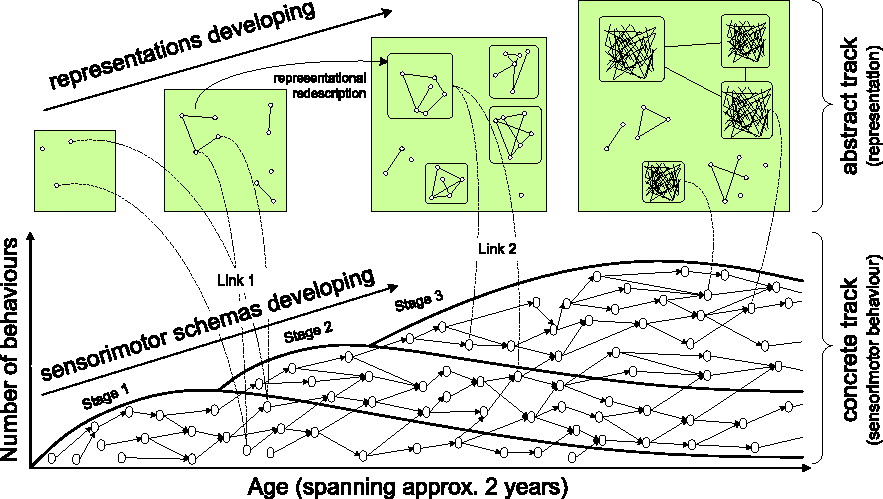
\includegraphics[width=\textwidth]{Figure_1_guerin.pdf}
	\caption{Conceptual diagram of infant development from \cite{guerin_survey_2013} Fig. 1.
	The lower (concrete) track shows a directed acyclic graph of sensorimotor schemas. 
	A node represents a newly created schema. 
	An edge has the meaning ``is a necessary precursor''. 
    Stage 1: behaviors without objects. 
    Stage 2: behaviors with single objects. 
    Stage 3: object-object behaviors. The schemas now involve relationship among objects, and locations and transforms within space.
    The higher (abstract) track represents representations of objects by schemas and physical properties influencing their interactions.} 
	\label{fig:general}
\end{figure}


Ziemke \cite{ziemke_construction_2001} examined how these views apply to robotics.
Oudeyer \cite{oudeyer_intrinsic_2007} stressed the importance of intrinsic motivation. 

\subsection{Drescher's}

Drescher notes that ``a constructivist account of the development of intelligence holds that the difference between the mind of an adult, and that of an infant, lies in mental structures built by the individual'' \cite[p. 41]{drescher_made-up_1991}.
He pioneered the first schema mechanism in 1991 by designing these mental structures as schemas formalized as the tuple (context, action, result) depicted in Fig. \ref{fig:drescher}. 
The \textit{context} and the results are sets of binary \textit{items} that can be \textit{positively} or \textit{negatively} included. 
A schema's context is satisfied when all the positively included items are \textit{On} and all the negatively included items are \textit{Off}. 
A schema's result asserts that, if the action is taken when the context is satisfied, then the positively included items of the results will be turned \textit{On} and its negatively included items will be turned \textit{Off}.

\begin{figure}
	\centering
	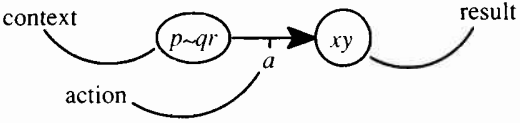
\includegraphics[width=0.6\textwidth]{Figure_2_schema_drescher.png}
	\caption{Schema from \cite{drescher_made-up_1991} Fig. 3.2.
		The schema noted $p \!\sim\! qr/a/xy$ asserts that if action $a$ is taken in the context where item $p$ is On, $q$ is Off, and $r$ is On then the items $x$ and $y$ will be turned On.} 
	\label{fig:drescher}
\end{figure}

The agent is initialized with a set of actions, \textit{primitive items}, and \textit{primitive schemas} that encode the agent's initial ``innate'' behaviors. 
The activation of a schema consists of initiating its action. An activated schema is said to \textit{succeed} if its predicted results are all in fact obtained, and to \textit{fail} otherwise. The ratio of success and failure is called \textit{reliability} and is memorized for each schema.  
As the agent interacts with its environment, it records new schemas that associate the observed context together with the action taken and the observed result. 
Schemas can be chained to achieve goals. 

Drescher implemented Piaget's idea of ``construction of reality'' through a mechanisms that seeks underlying invariant that make the enaction of some schemas reliable. 
The mechanism identifies \textit{relevant results} made of items that are slightly more frequent than average, 
and then seeks conditions under which the relevant results follow reliably. 
Such conditions are found through new schemas that allow recovering the context leading to the relevant result, and then performing the action again to asses the reliability of these new schemas. 
These new schemas act as ``probes'' that may evoke the manifestation of a ``thing''. 
They are only reliable if the ``thing'' is present. 
When such a schema is found, it is considered a ``host schema'' for a newly spawn ``synthetic item'' that represents this thing. 
Drescher notes that ``synthetic item thus works backward from a thing's manifestation to define the very thing manifested'' \cite[p. 83]{drescher_made-up_1991}.
This addresses the fundamental problem of \textit{concept invention} in that 
``a synthetic item is a new element of the system's ontology---an element fundamentally different from the prior contents of the system's conceptual vocabulary \cite[p. 81]{drescher_made-up_1991}.

The designer defines the agent's goals by assigning \textit{primitive values} to items.
The mechanism can identify subgoals as specific sets of items to be activated or deactivated; 
and it constructs \textit{composite actions} as sequences of schemas used to reach a subgoal.
Items also have \textit{instrumental values} and \textit{delegated values} that enter into play in the selection of schemas and composite actions.
The agent randomly alternates between explicit goal-pursuit and exploration, with probability defined by the designer.

%Drescher targeted the fundamental problem of \textit{concept invention} by implementing a mechanism to find underlying invariant 

%The new synthetic item is created in terms of primitive or previously created synthetic items.
%For example, returning the hand to where an object was last felt typically recovers the tactile manifestation of the object. A new concept is learned to represent this object. 

%This processes uses the mechanism's \textit{marginal attribution} facility, which ``use[s] sensitive statistical measures to alternate between discovering a highly unreliable result, and then seeking conditions with respect to which the result follows more reliably'' \cite[p. 5]{drescher_made-up_1991}.



% New items called \textit{synthetic items} are learned through a process called \textit{marginal attribution}.



\cite{chaput_constructivist_2004}
\cite{guerin_piagetian_2008}
\cite{wang_new_2012}
\cite{miller_building_2018}

\subsection{Perotto's}

Similar to Drescher's, Perotto's schemas \cite{perotto_computational_nodate} are tuples that associate a context, an action, and an expected result. 
Perotto, however, introduces a new distinction between two kinds of context variables: hidden variables and observable variables as shown in  Fig. \ref{fig:perotto}.

\begin{figure}
	\centering
	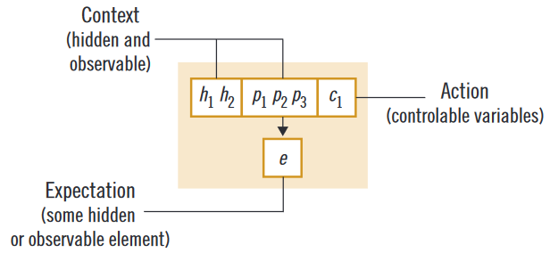
\includegraphics[width=0.6\textwidth]{Figure_perotto.png}
	\caption{Perotto's schema from \cite{perotto_computational_nodate} Fig. 2.
		A schema is composed of three vectors: context containing hidden variables and observable properties $(h_1, h_2, p_1, p_2, p_3)$, action $(c_1)$, and expected result $(e)$. } 
	\label{fig:perotto}
\end{figure}

Perotto also introduced a hierarchy of schemas called the \textit{anticipatory tree} represented in Fig. \ref{fig:perotto_tree}. 
Schema are organized in the \textit{anticipatory tree} whose top-level schema describes the agent's highest-level goal and leaf schemas are deciders of actions in the environment.

\begin{figure}
	\centering
	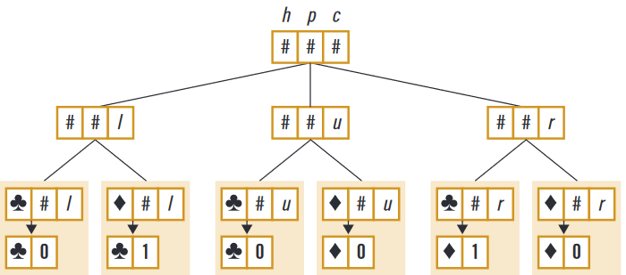
\includegraphics[width=0.7\textwidth]{Figure_perotto_tree.png}
	\caption{Example of Perotto's anticipatory tree from \cite{perotto_computational_nodate} Fig. 10: ``Final schematic tree for solving the flip problem.''.
 } 
	\label{fig:perotto_tree}
\end{figure}



\subsection{AERA}

AERA\footnote{Autocatalytic Endogenous Reflective Architecture; see www.openaera.org – accessed Dec. 6th, 2024.} is a unified system that can learn about causal relations cumulatively, from experience \cite{thorisson2019cumulative,thorisson2014autonomous,nivel2013autocatalytic}. The system’s knowledge representation uniquely combines ampliative reasoning, autonomous resource management, explanation-driven compositional knowledge representation and reflection in a synergetic architecture that can grow its knowledge from a small “bootstrapping seed” \cite{thorisson2020seed}. Its compositional knowledge contains numerous peewee-size “micro-models” that can be combined in explainable ways to model experience \cite{thorisson2021explanation}. 

The methodology behind AERA rests on three fundamental principles \cite{thorisson_seed-programmed_2020,thorisson2012new,nivel2009self}: 1. During learning, a learner autonomously creates new knowledge through a variety of methods including hypothesis generation and testing; 2. autonomous learning must create models of causal relations through situated goal-driven reasoning, and 3. self-programming is based on transparent operational semantics based on peewee-size uniform knowledge models. Those familiar with Piaget’s \cite{berlyne2003psychology} fundamental insight that human learning requires creation of new information will recognize the first principle. For this principle, Piaget proposed the idea of schemas – information structures that mediate between perception and action, capturing and controlling experience. An important difference between AERA’s knowledge representation and other proposals based on this idea (cf. \cite{arbib2003handbook,drescher_made-up_1991}) is its emphasis on non-axiomatic worlds and the resulting strong requirement for transversal defeasibility of acquired knowledge (cf. \cite{pollock1987defeasible}) – in other words, that since no certainty about anything learned can be guaranteed, the methods for knowledge creation cannot be based on the assumption of knowledge of a “ground truth”. The methodology behind AERA unifies this, and the above listed assumptions, in a coherent theoretical approach, with deep implications for knowledge creation in light of novelty: AERA starts out with only a tiny amount of “bootstrap” (seed) knowledge – the remainder of its knowledge, which soon vastly outsizes the seed\footnote{In our implementation of S1 – an AERA agent that learns to do TV-style interviews, the ratio of the learned knowledge over the seed knowledge, after 20 hours of learning, was ~53 \cite{thorisson2014autonomous}.}, is then generated autonomously by the system itself, based on hypotheses that are inspired and verified through experience, using ampliative reasoning mechanisms. 

\begin{itemize}
    \item The knowledge representation in AERA is peewee (relatively small) and compositional; AERA can inspect, deconstruct, and reconstruct its models, as well as create hierarchies of models of its experience.
    \item The models in AERA are falsifiable, have degrees of confidence, and can be related to specific groups with certain attributes specifying their context.
    \item The choice of models and reasoning methods at any point in time is dynamic, based among other things on the extent of available resources (models and time).

\end{itemize}



AERA’s peewee-size models, similar to e.g. Drescher’s \cite{drescher_made-up_1991} schemas and the neuro-symbolic approach presented in \cite{komrusch_symbolic_2022}, represent knowledge by contextualized programs that capture antecedental and successional states of important relationships (e.g. the relationship between a hand and an object that one wants to pick up). Unlike these, AERA places explicit representation of cause-effect relations at its core \cite{thorisson2018cumulative}. During its continuous learning, driven by a self-maintained dynamic goal hierarchy, the most useful (effective and efficient) models of cause-effect relations encountered in the environment are retained, while others are discarded. Based on predictions, informed experimentation, and strategic induction, the system autonomously creates new knowledge cumulatively, effortlessly unifying new information with old, even in light of contradictions. Further separating AERA from other approaches are its atomic elements for knowledge creation, whose operational semantics are transparent to the system’s own reasoning, meaning that they can be inspected and learned by the same explicit, defeasible unified reasoning mechanisms as used for learning about the world. 

The approach uniquely unifies cognition and meta-cognition in a single, coherent architecture, enabling efficient and effective self-reflection that lays a foundation for a capacity for cognitive growth. The result is a system that can dynamically employ ampliative reasoning, at any point in time, to predict both the immediate and far future, including its own cognitive resource use (“think time”). 

Key representational components of this approach include \cite{sheikhlar2024autonomous,sheikhlar2024causal}: 
\begin{itemize}
    \item \textbf{Facts} are statements that represent a cognitive event, e.g. operations happening in AERA itself; facts are the only entity in AERA that have complete certainty (corresponding to Descartes' axiom “I think, therefore I am”).
    \item A \textbf{composite State model (CST)} captures a set of simultaneous (timeless) Facts that the AERA system considers to be (potentially) useful and/or necessary for properly predicting an event’s consequences; used to e.g. represent a variety of subsets in the world such as spatial relations of objects, the values of a perceived object’s properties, such as its position and color, etc. %The forming of a CST at time T becomes a Fact with a timestamp T and a GUID (i.e. it is certain to the AERA executive that this CST was formed at time T). 
    \item A \textbf{cognitive event model (CEM)} captures a (hypothesized) causal influence of a Fact on another Fact; used to represent the effect that an action or event in particular circumstances, e.g. a command initiated by AERA at some timestep, has on the state of the world at a later timestep. When a CEM fires it produces a prediction (while the production of a prediction is represented as a Fact, the confidence in the prediction itself is defeasible and is in part based on the confidence of the CEM).
    \item A \textbf{requirement model ($M_{req}$)} captures the (predicted) requirements/conditions that must be met for a CEM to be relevant in a particular context at a particular time.

\end{itemize}


AERA’s programming paradigm allows the system itself to inspect these types of information structures, use them “for parts” to create variations, as well as create new ones from scratch. AERA’s programming language, Replicode, allows it to autonomously use these building blocks for self-programming, in the form of coherent plans, predictions, and goals that it can pursue \cite{nivel2013towards,nivel2013replicode,thorisson2012new}. These mechanisms have been demonstrated for control of virtual robots, language learning and use, and multimodal interaction \cite{thorisson2014autonomous,sheikhlar2024autonomous}). 

Both \textit{CEM}s and $M_{req}$s have a left-hand side (LHS) and a right-hand side (RHS), composed of sets of Facts and constraints (e.g., math equations). The LHS Facts describe (assumed) conditions under which the RHS Facts would be produced. Figure \ref{fig:AERA} shows how the above components lead to making a prediction. When some sensory Facts match everything in a \textit{CEM}’s LHS, a relevant $M_{req}$ allows the \textit{CTS}’s instantiation, which means the conditions for making a prediction via a \textit{CEM} are met. A successful instantiation of a \textit{CEM} means that everything in its RHS will happen  (probably – because all knowledge in AERA is defeasible). As the \textit{CEM} predicts a future state after an event’s occurrence, this is verified and marked as a “successful prediction” by AERA only if the prediction matches the state that is observed.

\begin{figure}
	\centering
	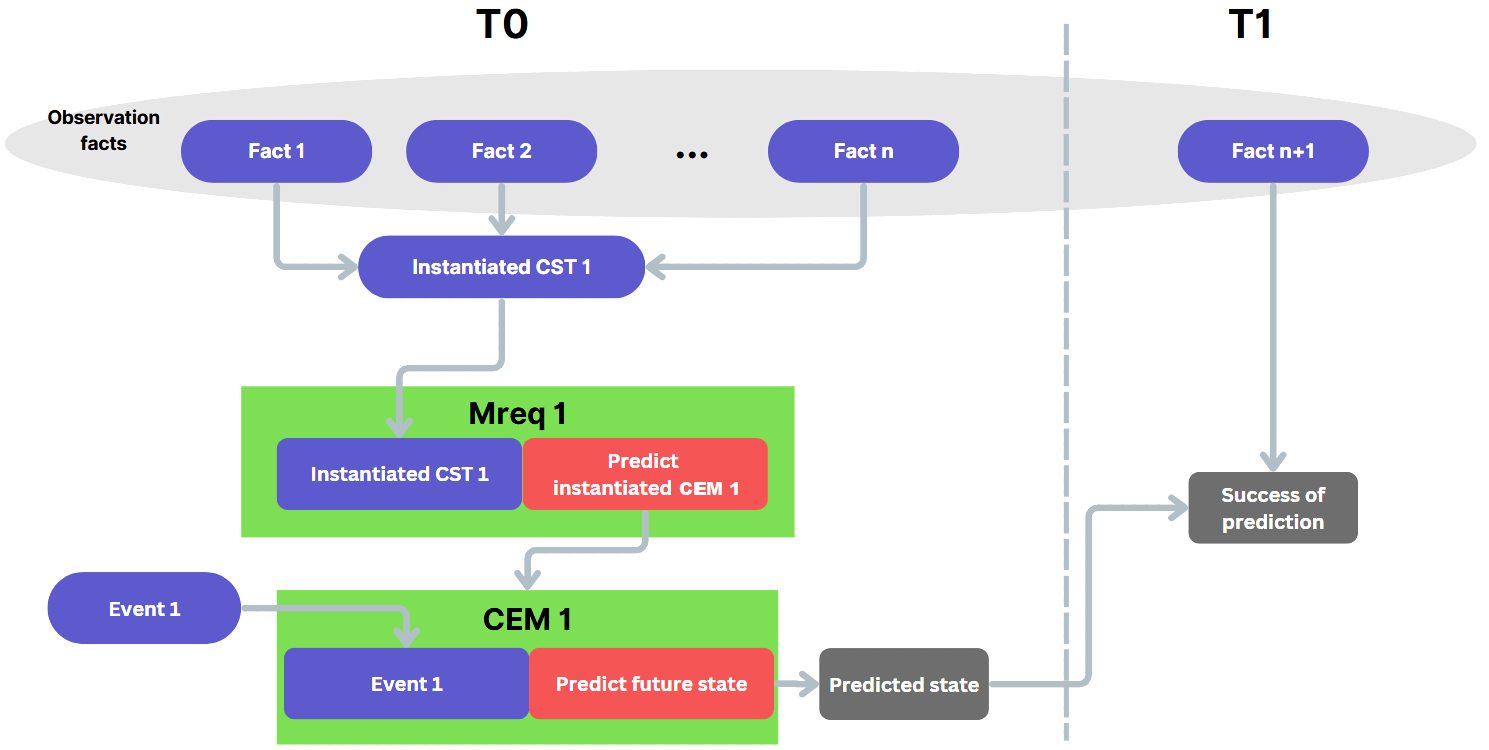
\includegraphics[width=0.99\textwidth]{AERAblockdiagram2.png}
	\caption{The connection between $CST$, $M_{req}$, and $CEM$. The observation facts matching $CST1$ allow $M_{req}$ to trigger a prediction by instantiating $CEM1$. AERA checks whether the subsequent observations match the predicted future state.} 
	\label{fig:AERA}
\end{figure}

As an example, the triad of $CST1$, $M_{req}1$, and $CEM1$ can represent the physical movement behavior of an entity when it collides with another entity (e.g., a hand). $CEM1$ represents the dynamics of the movement, connecting the collision event (left-hand side of $CEM1$) to the moved entity’s new position (right-hand side of $CEM1$). $CST1$ represents the preconditions of the behavior, such as the entities’ position, weight, etc., and the fact that the point of collision and the moved entities' position must initially be the same. $M_{req}1$ predicts that if a striking entity hits another entity with the conditions described by $CST1$, the stricken entity’s position will change a specific amount in the next time step.

The interactions of the operational principles of AERA are quite intricate in their entirety; important aspects that are covered elsewhere include induction – the creation of new knowledge – unified abduction-deduction – the creation of plans and explanations – and runtime relevance computations \cite{nivel2013towards}. The unified integration of these operational principles in a single coherent architecture is what gives AERA its power, allowing its seed – initial human-provided knowledge – to be orders of magnitude smaller than what AERA can create on its own through learning from experience. 


\subsection{The LIDA cognitive architecture}

The LIDA cognitive architecture \cite{kugele_learning_2021}  implements a schema mechanisms on top of a perceptual memory module called the Perceptual Associative Memory (PAM). 
Percepts are not directly received from the environment but constructed in the PAM through an active sensorimotor process. 
Other memory modules are implemented including episodic memory, declarative memory, and spatial memory.
Knowledge is represented as a directed graph called the \textit{node structure}. 

LIDA's schemas work as templates with unbound variables in their context, action, and result. 
Actions may have  unbound variables that qualify and modulate how an action is executed. 
Schemas are instantiated as \textit{behaviors}. 

LIDA implements \textit{affective valence}. 
Affective valence can bias behavior selection towards desirable outcome. 
Liking and disliking are distinguished from wanting and dreading with the argument that they relate to distinct neural pathways in the brain \cite{kringelbach_functional_2010}. 
Wanting and dreading are qualified by \textit{incentive salience} of behaviors.   

\begin{figure}
	\centering
	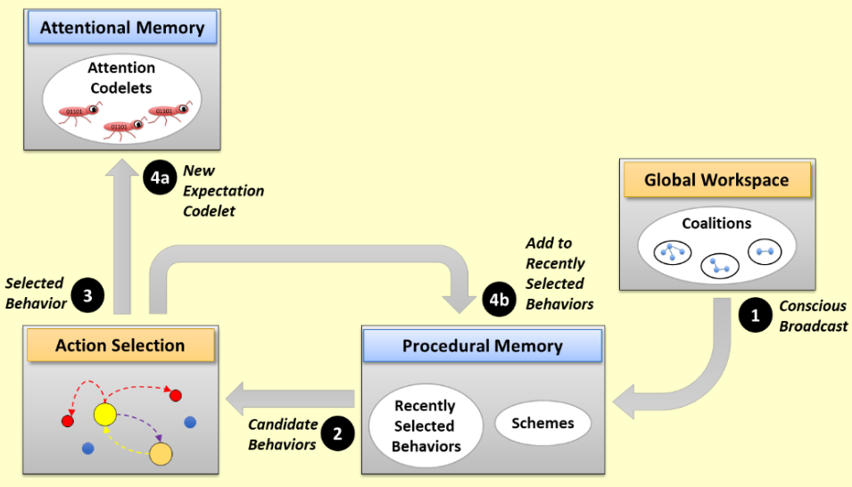
\includegraphics[width=0.7\textwidth]{Figure_LIDA1.png}
	\caption{Initiation of LIDA's procedural learning process (\cite{kugele_learning_2021} Fig. 10)} 
	\label{fig:lida1}
\end{figure}

\begin{figure}
	\centering
	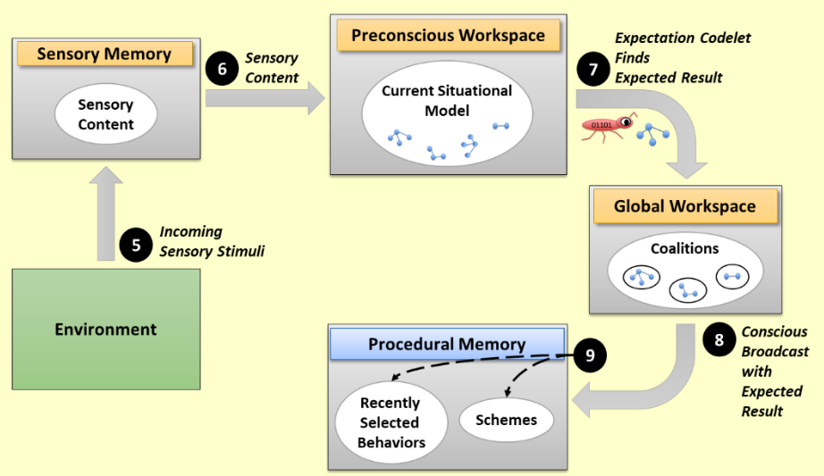
\includegraphics[width=0.7\textwidth]{Figure_LIDA2.png}
	\caption{Continuing process of selectionist and instructionalist procedural learning that was initiated by Action Selection (\cite{kugele_learning_2021} Fig. 11)} 
	\label{fig:lida2}
\end{figure}


\subsection{Georgeon's}

Similar to Perotto, Georgeon modeled schemas as tuples (pre-condition, decision, post-condition), and organized them  hierarchically. 

In contrast with Drescher's and Perotto's mechanisms, however, pre-conditions and post-conditions are not properties of the world (hidden or observed) but are other schemas learned previously. 
The mechanism learns new schemas from the bottom up, with higher-level schemas made of a sequence of two previously-learned lower-level schemas, 
as illustrated in Fig. \ref{fig:agent8}. 
The mechanism is not initialized with a top-level goal. 
Instead, it is initialized with a predefined set of low-level primitive schemas that define the agent's basic possibilities of interaction. 
In a robot, primitive schemas are hard-coded control loops involving actuators and sensory feedback. 


\begin{figure}
	\centering
	\includegraphics[width=1.0\textwidth]{Figure_3_agent8.pdf}
	\caption{Schema learning and selection.
		Schemas are nested tuples: (pre-schema, decision, post-schema).
		Over time, new decisions and new schemas are learned from the bottom up. 
		Recently enacted schemas (in gray) activate the previously-learned higher-level schema whose pre-schema they match.
		Activated schemas propose their post-schemas with a proclivity value calculated from the activation weight and the expected valence.
		The schema with the highest proclivity is selected to try to enact.} 
	\label{fig:agent8}
\end{figure}


The schema learning mechanism and selection works as follows.
At the end of time step $t$, the agent records or reinforces the schemas: 
\begin{itemize}
	\item[$\bullet$] $(i_{t-2}, d_{t-1}, i_{t-1})$
	\item[$\bullet$] $((i_{t-3}, d_{t-2}, i_{t-2}), d_{t-1}, i_{t-1})$
	\item[$\bullet$] $(i_{t-3}, d^2, (i_{t-2}, d_{t-1}, i_{t-1}))$
	\item[$\bullet$] $((i_{t-4}, d_{t-3}, i_{t-3}), d^2, (i_{t-2}, d_{t-1}, i_{t-1}))$
\end{itemize}

If it does not yet exist, the new decision $d^2$ is constructed different from the decision $d_{t-2}$ that was actually made at time $t-2$. 
For example, if the agent made decision $d_{t-2} = a0$ and enacted interaction $i_{t-2}=i00$, and then made decision $d_{t-1} = a0$, and enacted interaction $i_{t-1}=i01$, the agent learns the new decision $d^2=i00a0$ consisting of trying to enact the interaction $i_t=i00$ and then do action $a_{t+1}=a0$. 
When decision $d^2$ has been selected and successfully enacted, the mechanism learns higher-level schemas on top of it. 
The rate of schema construction being constant, the number of schemas grows linearly with time. 
Older and unused schemas can be forgotten.

In essence, the agent learns habits of interaction that are organized hierarchically, with shorter sequential habits learned first, and longer sequences of habits made of sequences of shorter habits later learned on top of them. 
Such habit learning relates to Woolford's \textit{sensorimotor sequence reiterator} \cite{woolford_precarious_2020}.

\section{Benchmarks}
\label{sec:benchmarks}

Fig. \ref{fig:drescher2} shows Drescher's experimental settings.


\begin{figure}
	\centering
	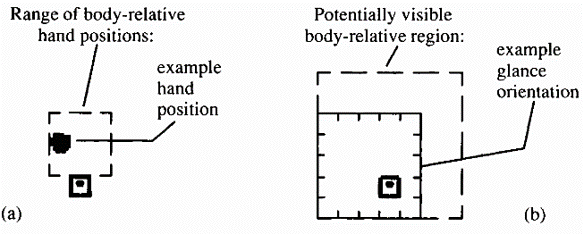
\includegraphics[width=0.6\textwidth]{Figure_drescher_expe.png}
	\caption{Drescher's benchmark from \cite{drescher_made-up_1991} Fig.6.1 ``Hand and glance ranges''.} 
	\label{fig:drescher2}
\end{figure}

Fig. \ref{fig:perotto_ben} shows Perotto's experimental settings \cite{perotto_computational_nodate}.


\begin{figure}
	\centering
	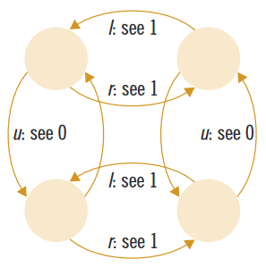
\includegraphics[width=0.3\textwidth]{Figure_perotto_benchmark.png}
	\caption{Perotto's benchmark from \cite{perotto_computational_nodate} Fig.9 ``The hyper-flip problem''.} 
	\label{fig:perotto_ben}
\end{figure}


\begin{figure}
	\centering
	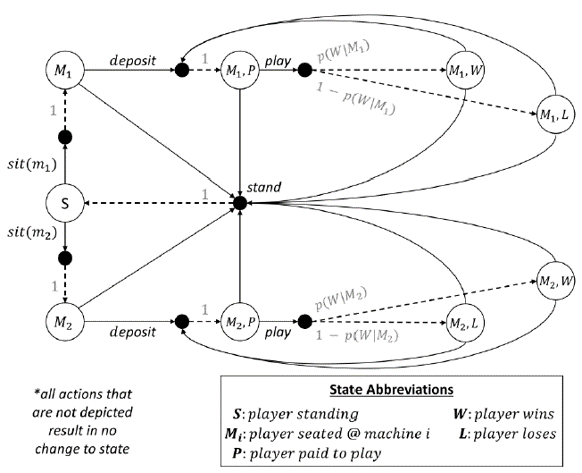
\includegraphics[width=0.7\textwidth]{Figure_LIDA_bench.png}
	\caption{The multi-armed bandit environment used to assess LIDA's schema Mechanisms (\cite{kugele_constructivist_nodate} Fig. 5)} 
	\label{fig:lida_bench}
\end{figure}



Fig. \ref{fig:georgeon} shows Georgeon' experimental settings \cite{georgeon_intrinsically-motivated_2012}.
This experimentation demonstrates a self-programming effect \cite{georgeon_cash_2019}.
Video Demo \cite{georgeon_video_2012}.


\begin{figure}
	\centering
	
\includegraphics[width=0.3\textwidth]{Figure_grid_plot.pdf}
	\caption{Georgeon's benchmark (Adapted from \cite{georgeon_intrinsically-motivated_2012}).
	The agent can move forward to an empty cell, bump into a wall (green cell), turn to the left or to right by 90°, or ``feel'' the cell in front, to the left, or to the right. 
	Sensory signal is a single-bit feedback from the action. 	
} 
	\label{fig:georgeon}
\end{figure}


\section{Schema mechanisms and theory of knowledge}

Table \ref{tab:comp} shows a comparison of the schema mechanisms presented in this paper.

\begin{table}
	\centering
	\caption{Comparison of schema mechanisms}\label{tab:comp}
	\begin{tabular}{|l|c|c|c|c|c|}
		\hline
		&  Drescher's & Perotto's & AERA & LIDA & Georgeon's \\
		\hline
		Chaining to goal & \checkmark & \checkmark & \checkmark & \checkmark &  \\
		Marginal attribution & \checkmark & \checkmark & \checkmark & \checkmark & \\
		Hierarchical goals &  & \checkmark & \checkmark &  &  \\
		Non-representational datum &  &  &  & \checkmark & \checkmark \\
		Intrinsic motivation &    &  &  & \checkmark & \checkmark \\
		Sequential schemas &    &  &  & \checkmark & \checkmark \\
		Active perception &    &  &  &  & \checkmark \\
		3D spatial schemas &    &  &  & \checkmark & \checkmark \\
		Reflexivity &    &  & \checkmark & \checkmark &  \\
		Defeasibility of acquired knowledge &    &  & \checkmark &  &  \\
		Self-programming &    &  & \checkmark &  & \checkmark \\
		\hline
	\end{tabular}
\end{table}



Bettoni  has criticized Drescher's schema mechanism in stating that ``Drescher's Constructivism is not Piaget's Constructivism, mainly because of its tacit acceptance of \textit{cognitive dogmatism}'' (\cite{bettoni_made-up_1993}, p. 6).
Bettoni describes cognitive dogmatism as taking for granted that ``patterns and structures of objects, attributes, relations, etc. [...] be as much as possible true copies of `original' objects, attributes, relations etc. in the world'' (\cite{bettoni_made-up_1993}, p. 1).
Indeed, theories of enaction as well as of radical constructivism have insisted that we should not take the sensory signals as representational items of an alleged reality. 


The game of Mastermind provides an emblematic example in which the observation is not representational. 
Player 2 attempts to infer a hidden combination of colored pegs (``hidden state'') by proposing guesses (``actions''), which Player 1 responds to with feedback pegs (``observation''). Black pegs indicate a correct color in the correct position, while white pegs indicate a correct color in the wrong position.
Since the observation depends on the action, there exist no function or stochastic distribution that map the state to the observation. 
The absence of such function or distribution is expressed in cognitive terms by that the observation is not ``representational'' of the state.

Software to play Mastermind have been proposed using diverse techniques such as entropy measure and evolutionary algorithms \cite{cotta_entropy-driven_2010}.
These techniques, however, require that the semantics of the feedback is known beforehand. 
We propose the \textit{constructivist Mastermind analogy} that likens a general learner to someone playing a giant game of mastermind where they start with no knowledge of the hidden combination and even the semantics of actions and feedback.
The player may never find the hidden combination or goal but may survive and strive for some time in a satisfactory \textit{knowledge niche}.

As reviewed in Section \ref{sec:benchmarks}, most schema mechanisms have been tested in settings in which the sensory signal is representational.
Nonetheless, the fact that they have not been tested with non-representational sensory signal does not mean that they would not work or could not be adapted to such settings. 
Georgeon's mechanism may constitute an illustration of that.  
In Georgeon's schemas, the sensory data is feedback from action rather than beeing representational. 
The pre-condition and post-condition of schemas are are just other schemas all the way down to non-representational primitive schemas. 
In essence, the agent knows its current context by possibilities of interaction rather than by representational data. 

Georgeon's schema mechanism is not targeted at reaching a predefined goal. Since sensory data does not represent the environment's state, the agent cannot have a goal represented as an environment state. Instead, the agent's behavior is driven by the expected valence of each decision. 
The calculation of expected valence may incorporate predefined preferences for some primitive schemas or different intrinsic motivation principles such as an estimation of information gained. 

\section{Conclusion}

Beyond the first stage called by Piaget the \textit{sensorimotor level}, comes a second stage he calls the \textit{first level of pre-operative thought} (\cite{piaget_lepistemologie_2011}, p. 30). 
It is at this second stage that the subject begins to differentiate itself from the objects. 
The subject becomes able to manipulate the schemas by thought. 
Piaget formulates this process as follows: 
\\

\begin{adjustwidth}{1cm}{1cm}
``On top of simple actions that ensure direct interdependence between the subject and objects, in certain cases, a new type of action is superimposed, one that is internalized and more precisely conceptualized: for example, in addition to being able to move from A to B, the subject acquires the ability to mentally represent this movement from A to B and to evoke, through thought, other movements'' (translated from \cite{piaget_lepistemologie_2011}, p. 30).\\

\end{adjustwidth}

Future studies on schema mechanisms will have to address this second stage to tackle fundamental questions of knowledge abstraction. 
We expect this will involve a cognitive architecture that has the capacity to represent spatial properties of schemas, and to simulate the enaction of schema in different spatial frames of reference. LIDA and ECA \cite{georgeon_artificial_2024} constitute initial attempts in this direction . 


\begin{credits}
\subsubsection{\ackname} .

\subsubsection{\discintname}
The authors have no competing interests to declare that are
relevant to the content of this article.
\end{credits}
%
% ---- Bibliography ----
%
% BibTeX users should specify bibliography style 'splncs04'.
% References will then be sorted and formatted in the correct style.
%
\bibliographystyle{splncs04}
\bibliography{ConstructivistAI.bib}
%
\end{document}
